\chapter{Mixed: Integer Programming}
This lecture is not in scope. \\
In this chapter, we will be discussing non-linear, integer programming, such that we may step into the non-linear regime of optimization via techniques that we have built up in this class so far. \\
As a personal note, in the adversarial machine learning project of EECS 127, we have seen problems (such as finding images with discrete values for pixels) that require integer outputs.

\section{Integer Programming}
In integer programming, our objective need have integer constraints: the solution must be an integer.
These problems are generally phrased as:
\[
    p^* = \min_{
        \substack{
            A \vec{x} = \vec{b} \\
            \vec{l} \leq \vec{x} \leq \vec{u} \\
            x_j \in \Z
        }
    } \vec{c}^T \vec{x}
\]
An integer decision variable comes in many contexts. \\
For example, an indicator variable itself is an integer decision variable (where $1$ expresses ``True'', $0$ expresses ``False'').
A mixed integer program, meanwhile, is an integer program that also involves floating number decision variables.

Let us explore integer programming with an example problem below.

\subsection{Exploration by Example}
Suppose UC Berkeley wants to build new buildings. It can build new buildings, or new dorms. \\
Both buildings and dorms can be built on either southside or northside, but we want to build at most one dorm, and if we build a dorm it should be close to buildings.
We observe constraints, but they are more qualitative than quantitative, but as in any optimization value, we will handle this optimization problem by expressing the value and cost of each investment:
\begin{center}
    \begin{tabular}{c|c||c|c||c}
        Building Type & Location & Value & Cost & Representative Variable \\
        \hline
        \hline
        Building & North & 9M & 6M & $x_1 \in \{0, 1\}$ \\
        & South & 5M & 3M & $x_2 \in \{0, 1\}$ \\
        \hline
        Dorm & North & 6M & 5M & $x_3 \in \{0, 1\}$ \\
        & South & 4M & 2M & $x_4 \in \{0, 1\}$
    \end{tabular}
\end{center}
Suppose our budget is 10M, then we may mathematically phrase this optimization as follows:
\[
    \max_{
        \substack{ 
            \forall i, 0 \leq x_i \leq 1 \land x_i \in \Z \\
            6x_1 + 3x_2 + 5x_3 + 2x_4 \leq 10 \\
            x_3 + x_4 \leq 1 \\
            x_3 = 1 \implies x_1 = 1 \\
            x_4 = 1 \implies x_2 = 1
        }
    } 9x_1 + 5x_2 + 6x_3 + 4x_4
\]
As a side note, $x_3 = 1 \implies x_1 = 1$ states one of the constraints above, that ``if we build a dorm it should be close to buildings''.
Now, let us further simplify such constraint into:
\[
    x_3 - x_1 \leq 0
\]
Because:
\begin{itemize}
    \item In the case that $x_1 = 1$, our expression $x_3 - x_1$ is $0$.
    \item In the case that $x_3 = 0$, our expression $x_3 - x_1$ must be negative.
    \item The only case at which this value becomes positive is that $x_3 = 1, x_1 = 0$, but that is against the implication.
\end{itemize}
Along such logic, we may then rephrase our problem as:
\[
    \max_{
        \substack{ 
            \forall i, x_i \in \{0, 1\} \\
            6x_1 + 3x_2 + 5x_3 + 2x_4 \leq 10 \\
            x_3 + x_4 \leq 1 \\
            x_3 - x_1 \leq 0 \\
            x_4 - x_2 \leq 0
        }
    } 9x_1 + 5x_2 + 6x_3 + 4x_4
\]

\section{Disjunction of Constraints}
The application of integer programming is wide.
For example, as indirectly demonstrated above, enables us to write ``either/or'' expressions within the constraint.

Suppose we attempt to express the following constraint in an optimization problem:
\[
    3x_1 + 2x_2 \leq 18 \oplus x_1 + 4x_2 \leq 16
\]
\textit{Note, $\oplus$ stands for either-or, and is mathematically called ``xor''.}

We can rephrase the above constraint by introducing a large constant $M$. \\
Now, for a binary variable $y$, I reexpress my constraint as follows:
\[
    \begin{cases}
        3x_1 + 2x_2 \leq 18 + yM \\
        x_1 + 4x_2 \leq 16 + (1 - y) M
    \end{cases}
\]
that way, introducing the binary variable $y$ lets us toggle between different constraints on an either-or fashion.

When we have more constraints within the xor sequence, we will make a decision tree of constraints via multiplying more binary variables.

\section{Algorithmic Works}
Integer Programs are useful not just for the above capabilities.
It also has the following properties:
\begin{bindenum}
    \item There are few feasible solutions. However, this number can explode very quickly, essentially exponentially in number of decision variables.
    \item However, with more constraints, integer programs can lead to faster solutions.
\end{bindenum}

Integer programs have many solving softwares, such as Cplex and Gurobi.
They use an algorithm known as ``Branch and Bound'' (Land and Dong, 1960s), which is still the state-of-the-art strategy for solving these programs.

\subsection{Demonstration of BB Algorithm}
Let us attempt solving the aforementioned building problem with Branch and Bound Algorithm.

We would begin by solving the optimization problem without the integer constraint on decision variables.
In such effort, we acquire that:
\[
    \begin{cases}
        p^* = 16.5 \\
        \vec{x}^T = \begin{bmatrix} 0.833 & 1 & 0 & 1 \end{bmatrix}
    \end{cases}
\]
We see that such solution is infeasible.
One simple solution to bring back the integer constraint is to round a decision variable; however, in doing so, we may violate other constraints.
What we perform instead, then, is to build a branch on the non-integral decision variable: $x_1$. \\
Consider a branch of the problem based on the value of $x_1$, such that for branches $b_0, b_1$:
\[
    p_{b_i}^* = \max_{
        \substack{
            x_1 = 0 \\
            other constraints as is
        }
    } f_0(x)
\]
we solve such linear program without integer constraints again.
In such case, we find our incumbent solution as follows:
\[
    \begin{cases}
        p_{b_0}^* = 9 \\
        \vec{x}^T = \begin{bmatrix} 0 & 1 & 0 & 1 \end{bmatrix}
    \end{cases}
\]
Meanwhile, on the other branch we would find:
\[
    \begin{cases}
        p_{b_1}^* = 16.2 \\
        \vec{x}^T = \begin{bmatrix} 1 & 0.8 & 0 & 0.8 \end{bmatrix}
    \end{cases}
\]

As we encounter non-integral solutions, we continue to traverse along such direction (because there's no branches that is supposed to occur under integral solutions).
The overall operation of our BB efforts is as traced follows:
\begin{center}
    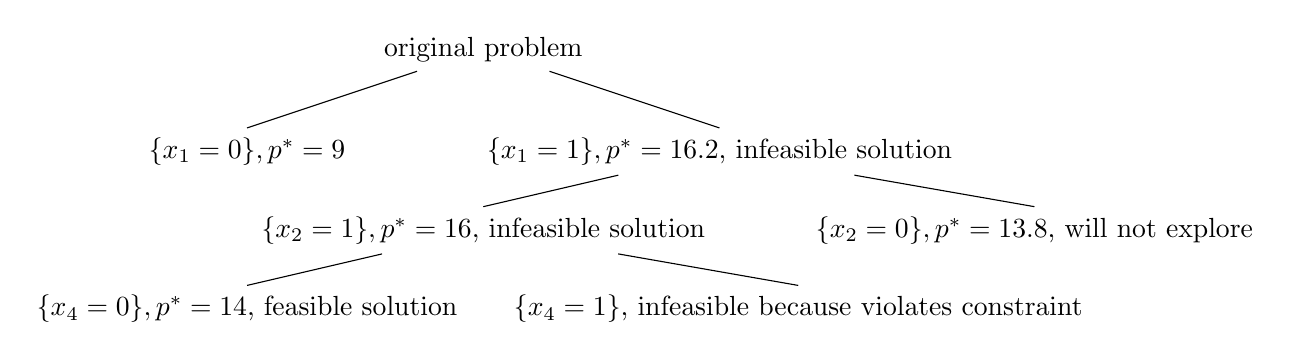
\begin{tikzpicture}
        \node (A) at (0, 0) {\text{original problem}};
        \draw (A) -- (-3, -1) node[below] (b11) {$\{x_1 = 0\}, p^* = 9$};
        \draw (A) -- (3, -1) node[below] (b12) {$\{x_1 = 1\}, p^* = 16.2$, \text{infeasible solution}};
        \draw (b12) -- (7, -2) node[below] (b21) {$\{x_2 = 0\}, p^* = 13.8$, \text{will not explore}};
        \draw (b12) -- (0, -2) node[below] (b22) {$\{x_2 = 1\}, p^* = 16$, \text{infeasible solution}};
        \draw (b22) -- (-3, -3) node[below] (b31) {$\{x_4 = 0\}, p^* = 14$, \text{feasible solution}};
        \draw (b22) -- (4, -3) node[below] (b32) {$\{x_4 = 1\}$, \text{infeasible because violates constraint}};
    \end{tikzpicture}
\end{center}
We make the conclusion that the incumbent solution is determined at the branch of $x_4 = 0$.

We did not explore the branch of $x_2 = 0$ because as we traverse the tree, the value of $p^*$ only becomes smaller (since we are exploring sub-optimal values that are less than their non-integer optimization results).
If the branches only yield smaller variables, we don't explore it.
More specifically, we should recognize that the primitive version of BB is a depth-first-traversal algorithm, and we ended up finding $p^* = 14$ before encountering the $x_2 = 0$ branch that has a smaller argument, therefore pruned that branch. \\
That means, if we have to explore the $x_2 = 0$ branch first, we would actually explore that branch because we didn't find a better maximum than $9$, the first incumbent solution, yet.
